\chapter{Notações Utilizadas em Redes Neurais} \label{apendice:notacao}
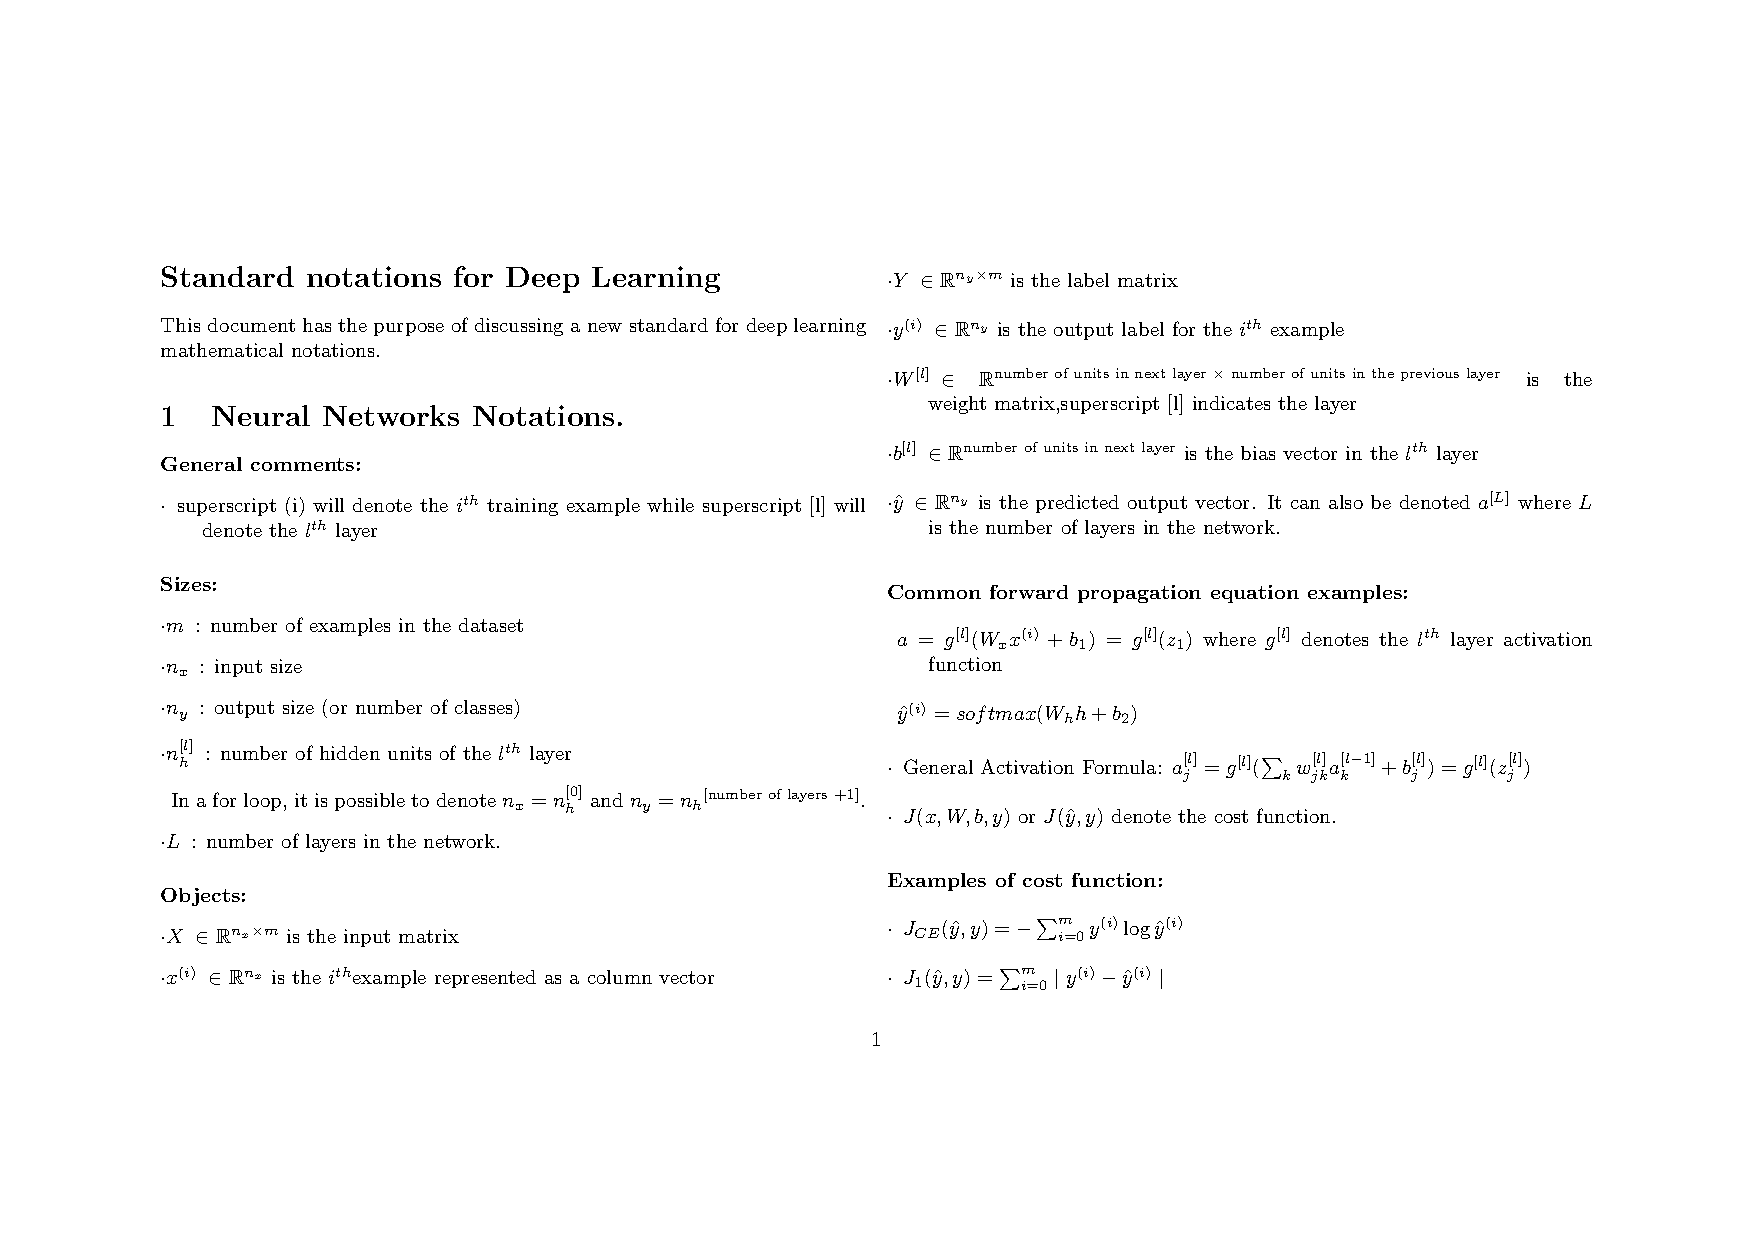
\includepdf[pages={1}, landscape=true]{pdf/deep-learning-notation.pdf}


\chapter{Etapas De Treinamento Utilizando a Rede Neural YOLO } \label{apendice:etapas-yolo}
\begin{itemize}
  \item Criar o arquivo ``yolo-obj.cfg'' com o mesmo conteúdo de ``yolov4-custom.cfg'';
  \item Alterar ``yolo-obj.cfg'' para:
  \begin{itemize}
    \item Considerar \textit{batches} com 64 imagens, onde um \textit{batch} representa o número de amostras a serem trabalhadas antes de atualizar os parâmetros do modelo \cite{ref:Brownlee};
    \item Subdividir cada \textit{batch} em 16 imagens (para processamento paralelo em treinamentos utilizando GPUs - Unidade de Processamento Gráfico do inglês \textit{Graphics Processing Unit});
    \item Utilizar um número máximo de \textit{batches} igual ao produto $n_{classes} \cdot 2000$
    \item Alterar o número de passos de acordo com o número máximo de \textit{batches};
    \item Alterar a quantidade de filtros considerando a fórmula $(n_{classes} + 5) \cdot 3$.
  \end{itemize}
  \item Criar o arquivo ``obj.names'' com os nomes das classes utilizadas, com cada nome em uma linha nova;
  \item Alterar no arquivo ``obj.data'' o número de classes utilizadas;
  \item Colocar as imagens de treinamento e teste no diretório ``obj'' que se encontra dentro de ``data'';
  \item Criar um arquivo de texto com a extensão ``.txt'' para cada uma das imagens do \textit{dataset} no mesmo diretório em que elas estão contendo os objetos e suas respectivas coordenadas, seguindo o padrão  $<objectclass> <x_{center}> <y_{center}> <width> <height>$ de forma que cada linha represente um objeto, onde
  \begin{itemize}
    \item $<objectclass>$ indica a classe do objeto de acordo com a ordem definida no arquivo ``obj.names'' com valores dentro do intervalo $[0, n_{classes} - 1]$;
    \item $<x_{center}> <y_{center}>$ são as coordenadas centrais da localização da caixa delimitadora do objeto, valores em ponto flutuante dentro do intervalo $[0.0, 1.0]$, normalizados de acordo com o tamanho da imagem utilizada.
    \item $<width> <height>$ são a largura e a altura, respectivamente, da caixa delimitadora do objeto, valores em ponto flutuante dentro do intervalo $[0.0, 1.0]$, normalizados de acordo com o tamanho da imagem utilizada.
  \end{itemize}
  \item Criar os arquivos de texto ``train.txt'' e ``test.txt'' que contém o nome das imagens utilizadas no treinamento e teste, respectivamente, onde para cada imagem utiliza-se uma nova linha;
  \item Fazer o \textit{download} de pesos pré-treinados, com intuído de acelerar o treinamento;
  \item Iniciar o treinamento.
\end{itemize}


\chapter{Placas de Circuito Impresso Utilizadas para o Conjunto de Dados HRIPCB} \label{apendice:hripcb-pcbs}

\begin{figure}[!h] %H
  \centering
  \caption{PCI Número 01 do conjunto de dados HRIPCB.}
  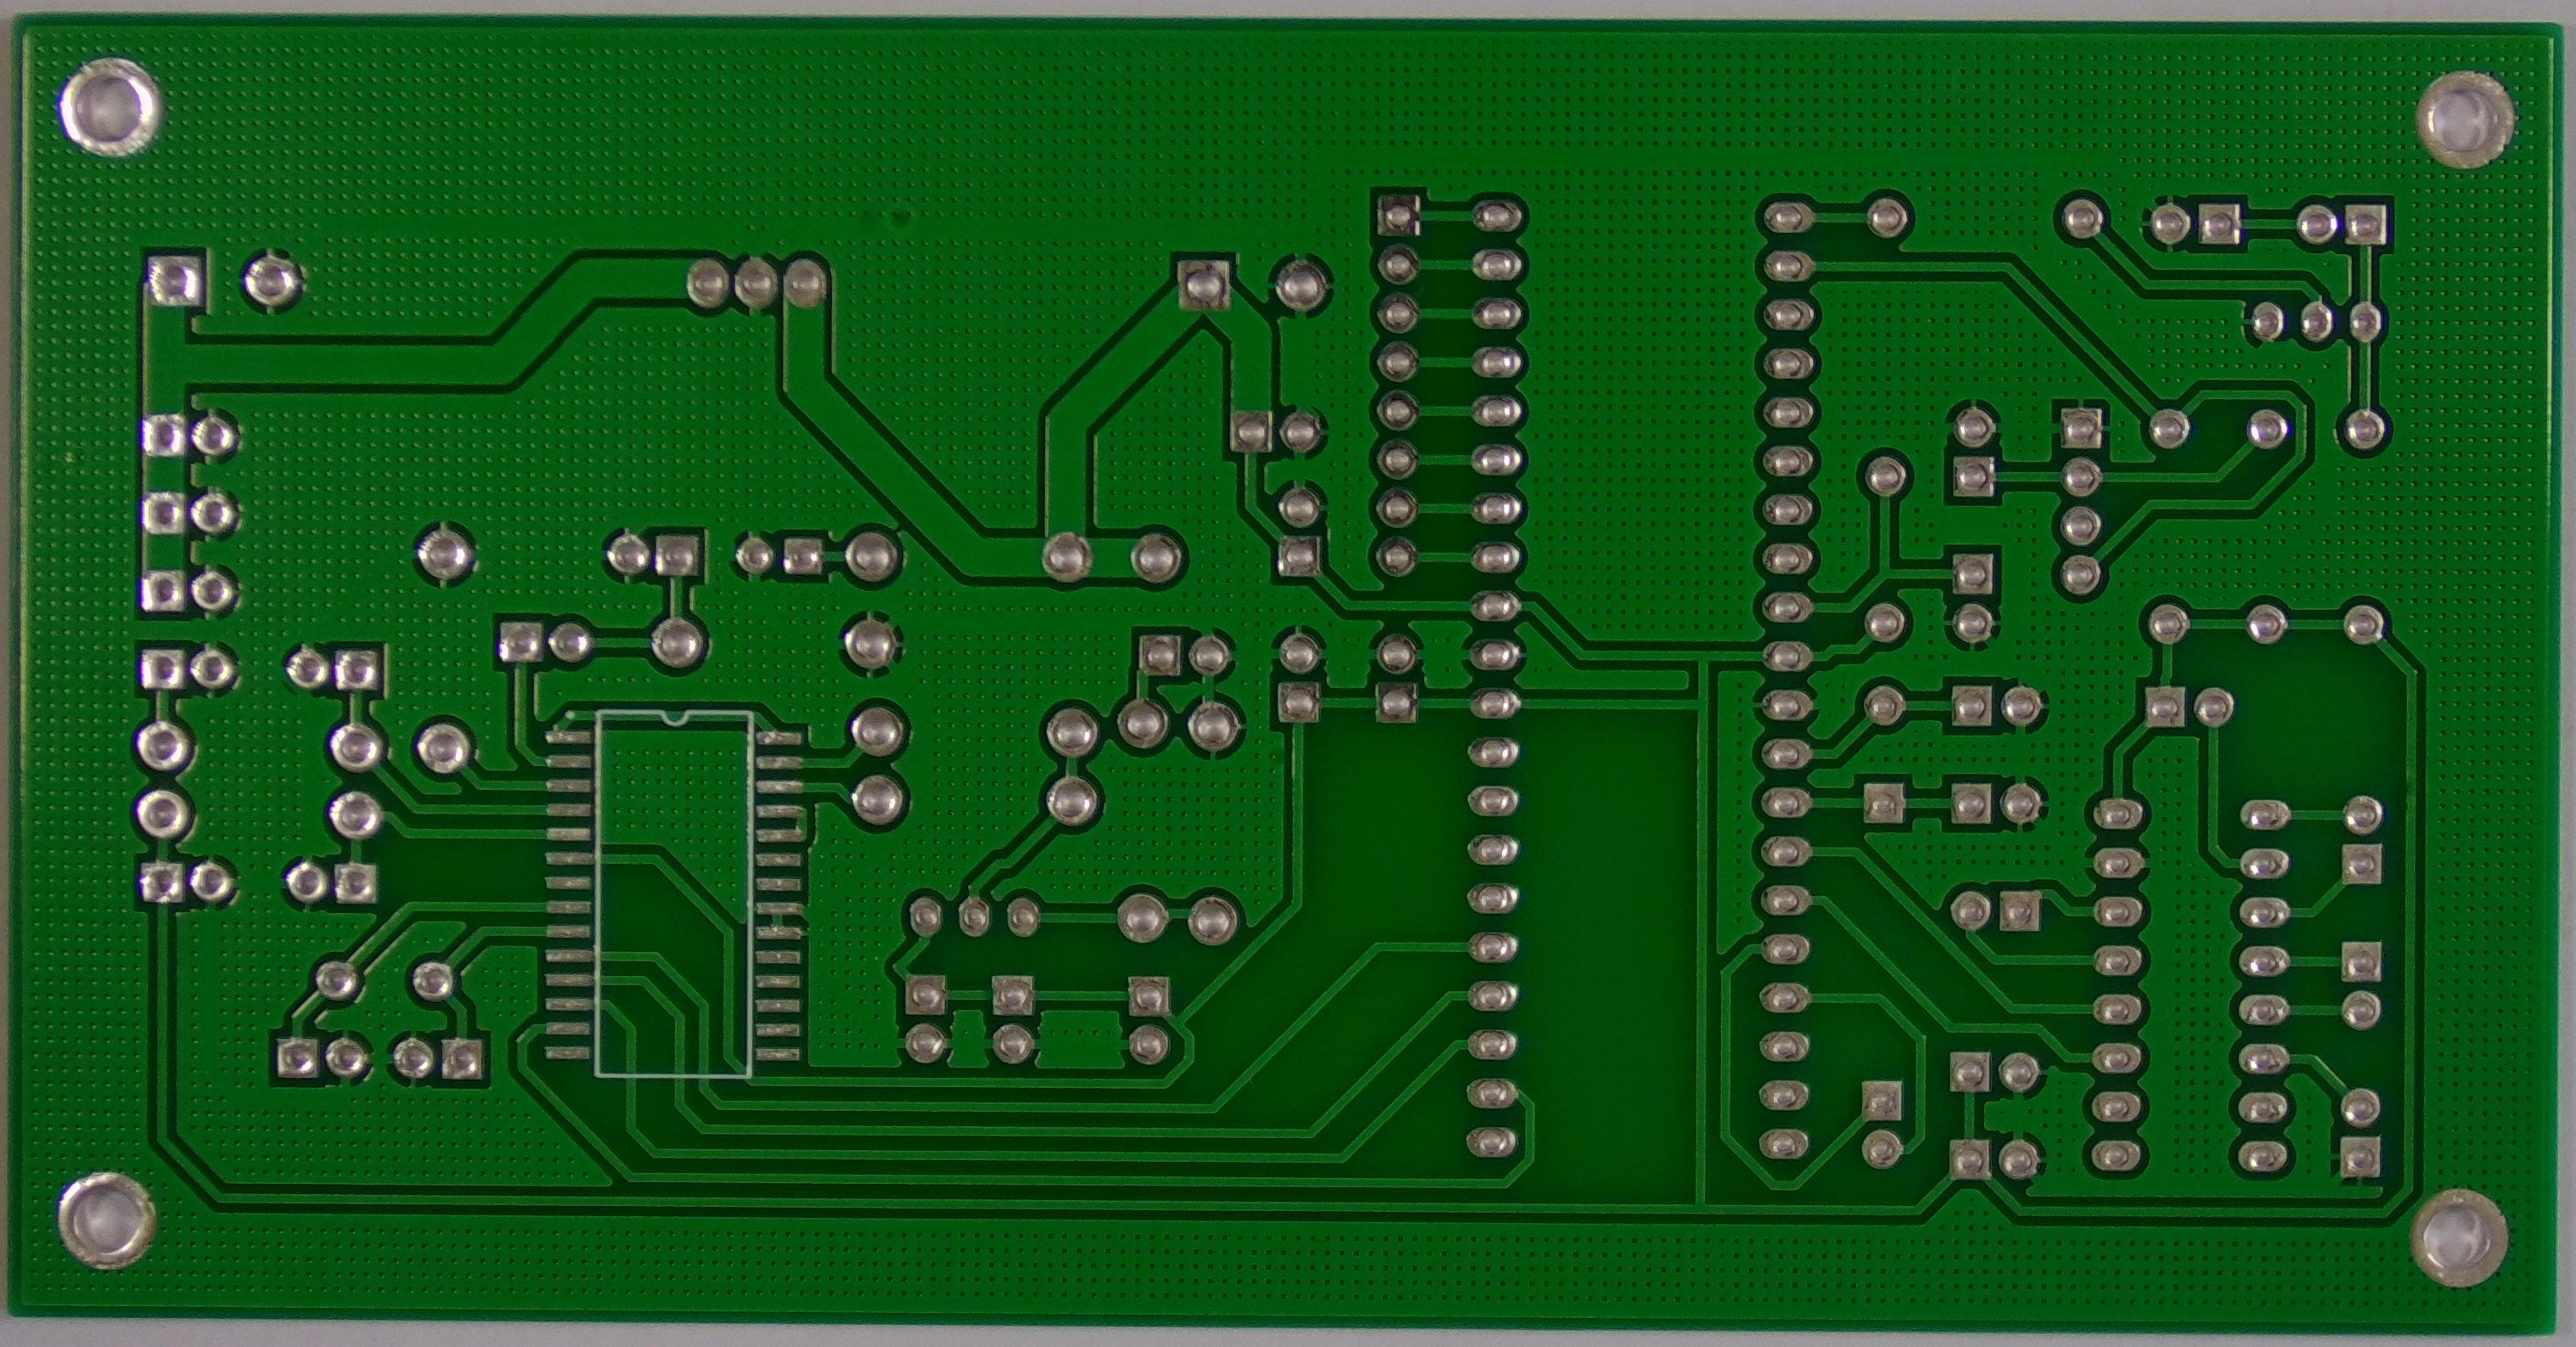
\includegraphics[scale=0.11]{img/pcbs/01.JPG}
  \label{fig:ap-pcbs-1}
  \indentedfont[15.2cm]{\citeonline{ref:Huang-et-al}}
\end{figure}

\begin{figure}[!h] %H
  \centering
  \caption{PCI Número 04 do conjunto de dados HRIPCB.}
  \includegraphics[scale=0.11]{img/pcbs/04.JPG}
  \label{fig:ap-pcbs-4}
  \indentedfont[15.2cm]{\citeonline{ref:Huang-et-al}}
\end{figure}

\begin{figure}[!h] %H
  \centering
  \caption{PCI Número 05 do conjunto de dados HRIPCB.}
  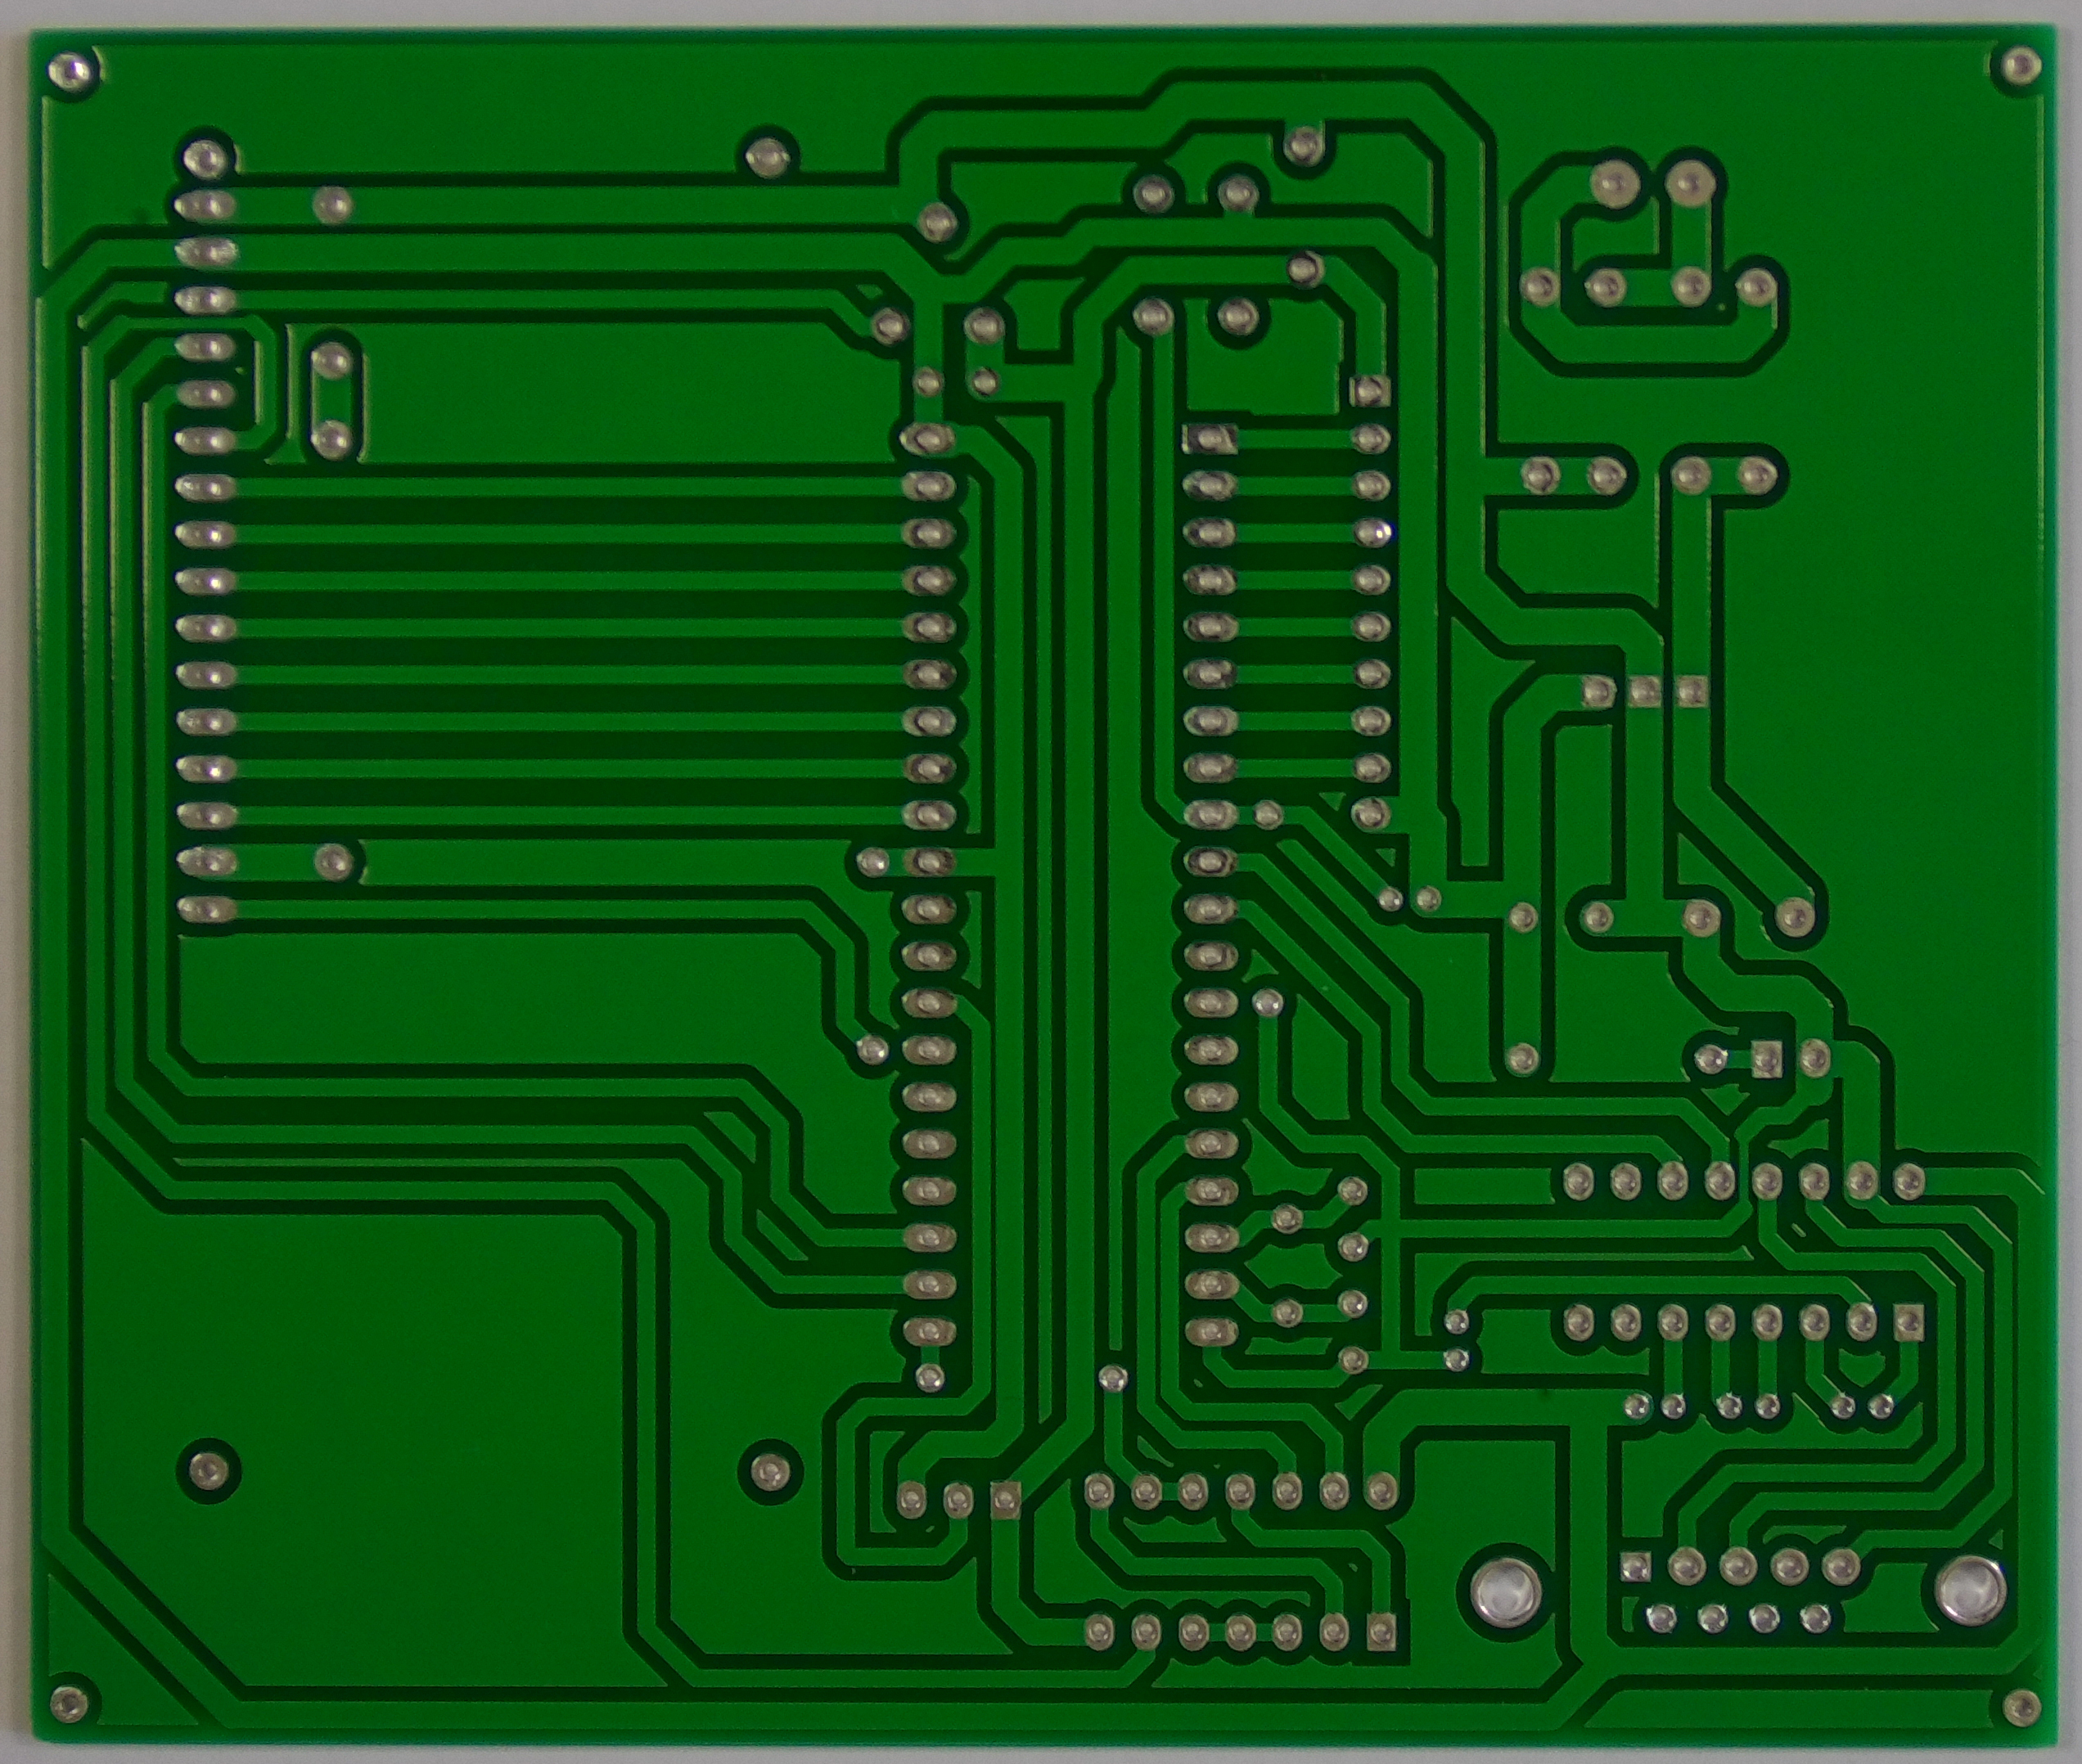
\includegraphics[scale=0.13]{img/pcbs/05.JPG}
  \label{fig:ap-pcbs-5}
  \indentedfont[15.2cm]{\citeonline{ref:Huang-et-al}}
\end{figure}

\begin{figure}[!h] %H
  \centering
  \caption{PCI Número 06 do conjunto de dados HRIPCB.}
  \includegraphics[scale=0.13]{img/pcbs/06.JPG}
  \label{fig:ap-pcbs-6}
  \indentedfont[15.2cm]{\citeonline{ref:Huang-et-al}}
\end{figure}

\begin{figure}[!h] %H
  \centering
  \caption{PCI Número 07 do conjunto de dados HRIPCB.}
  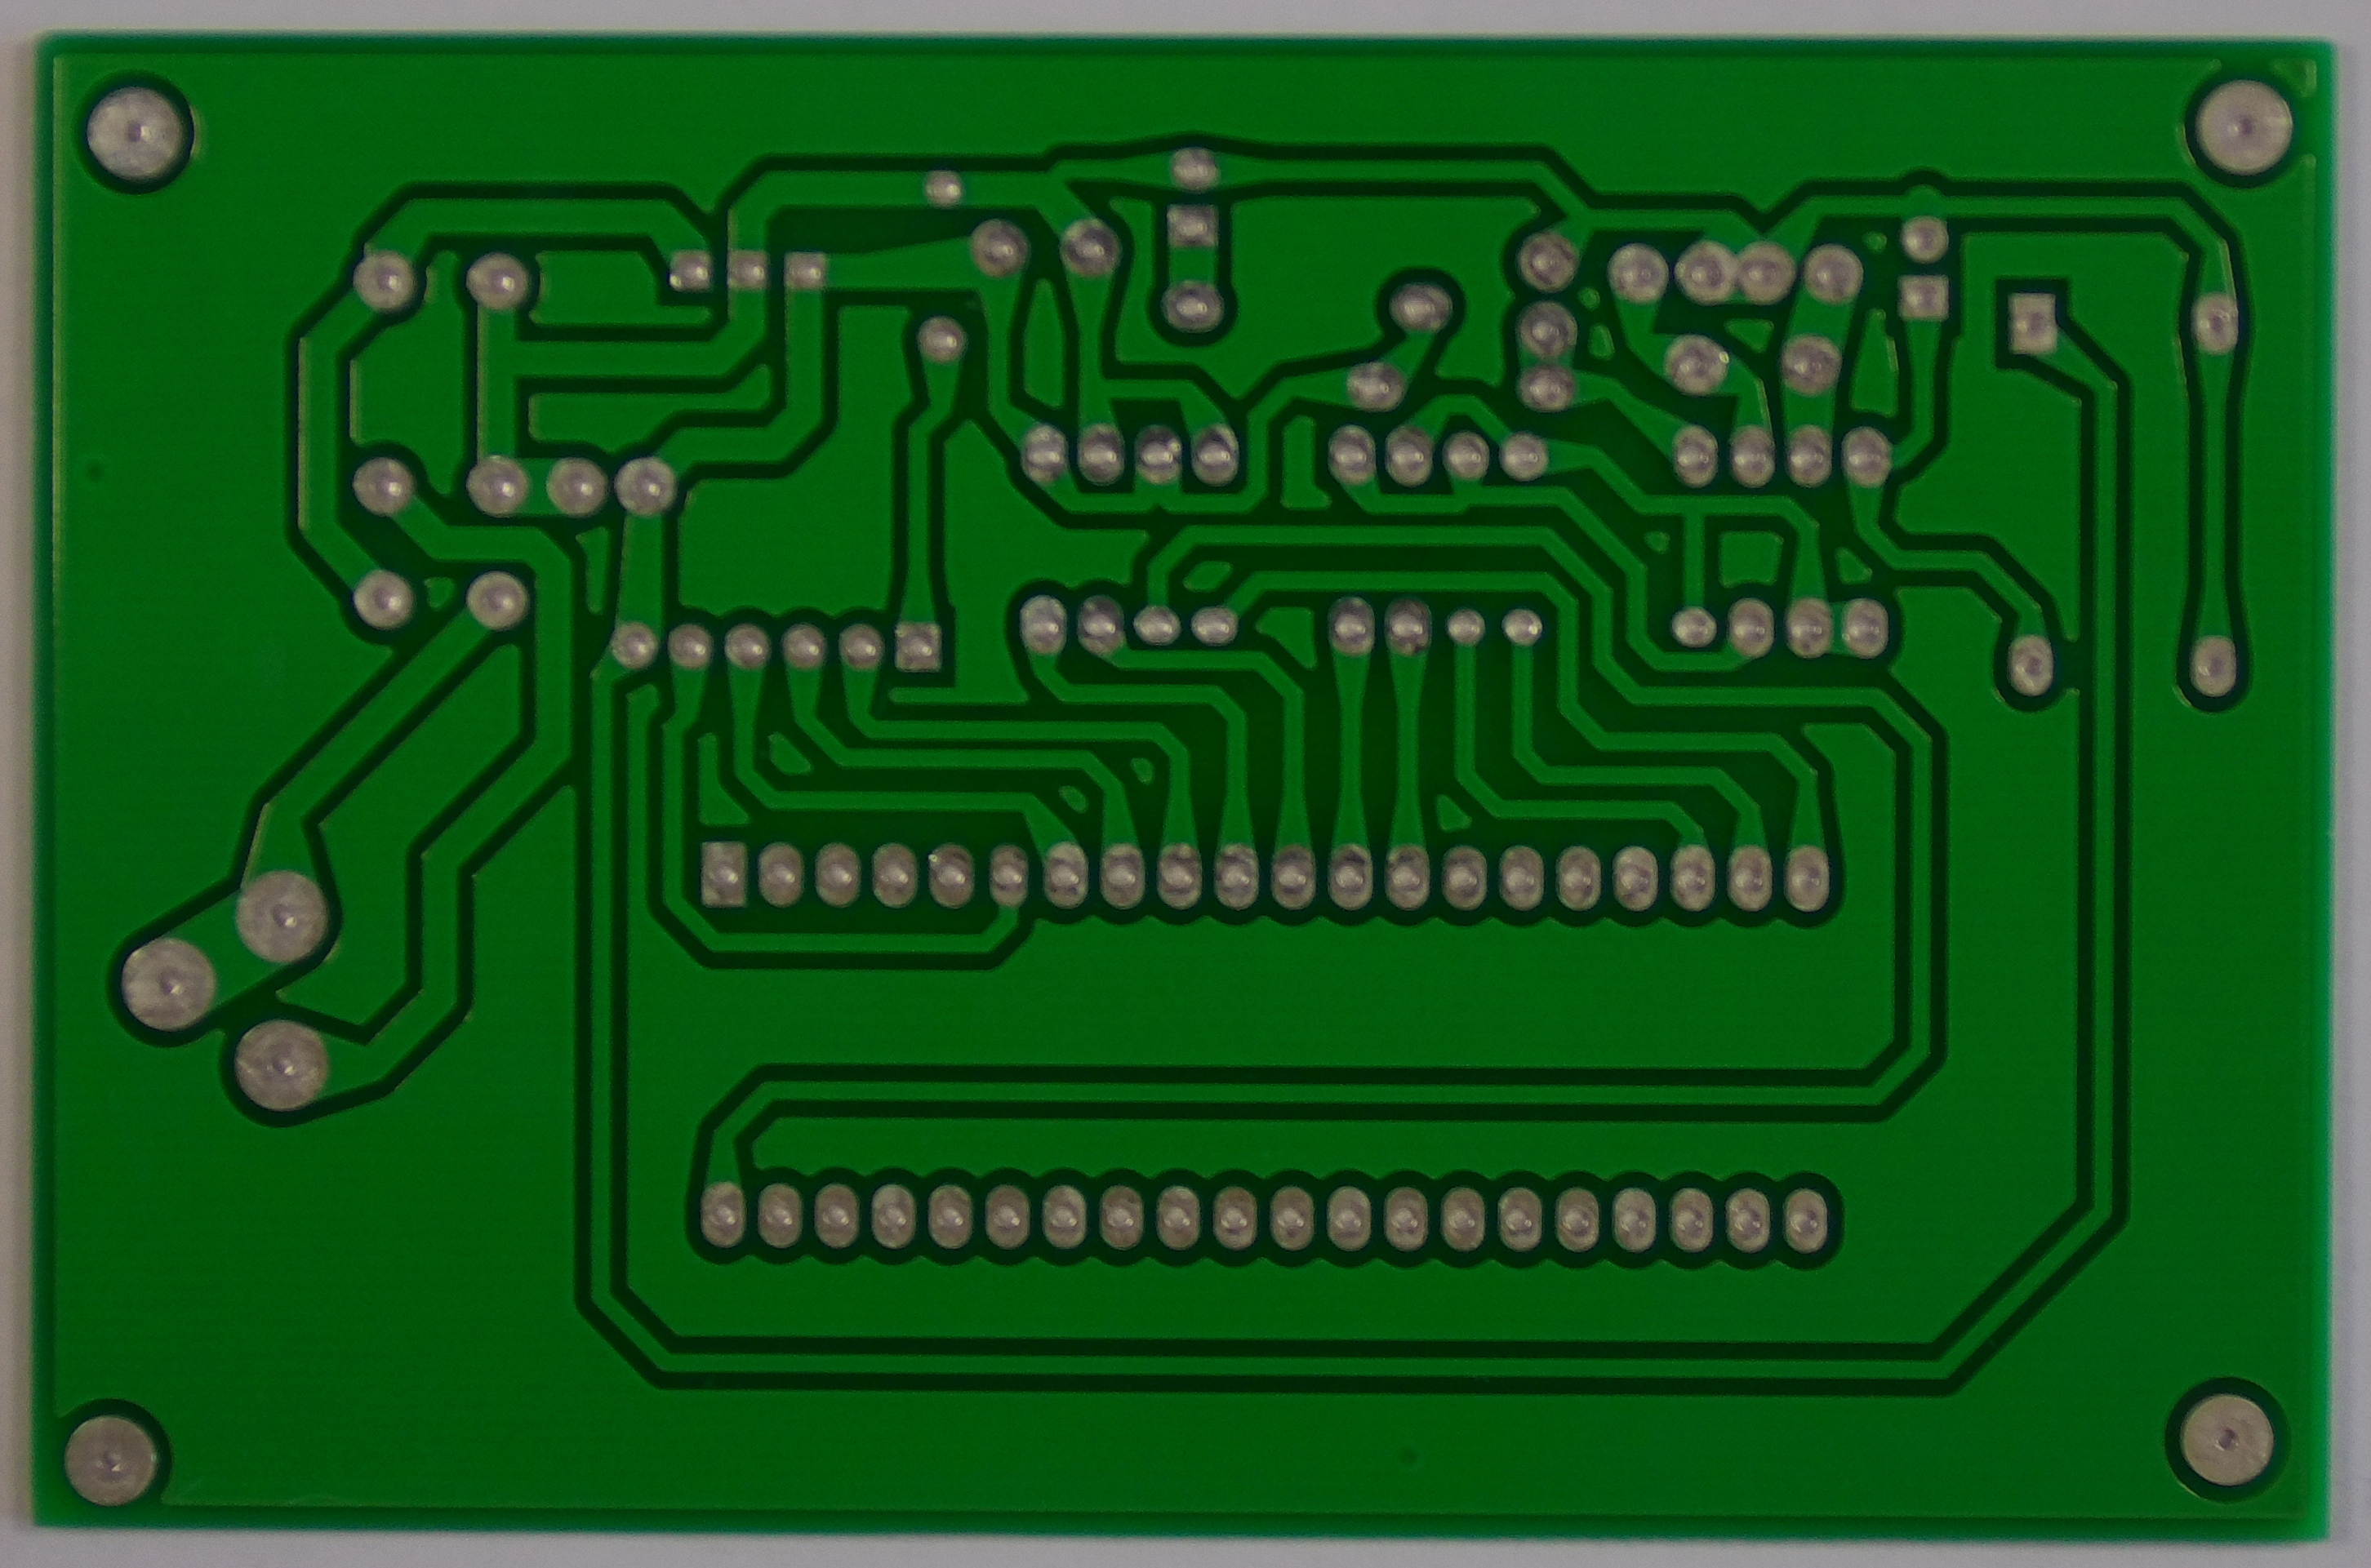
\includegraphics[scale=0.13]{img/pcbs/07.JPG}
  \label{fig:ap-pcbs-7}
  \indentedfont[15.2cm]{\citeonline{ref:Huang-et-al}}
\end{figure}

\begin{figure}[!h] %H
  \centering
  \caption{PCI Número 08 do conjunto de dados HRIPCB.}
  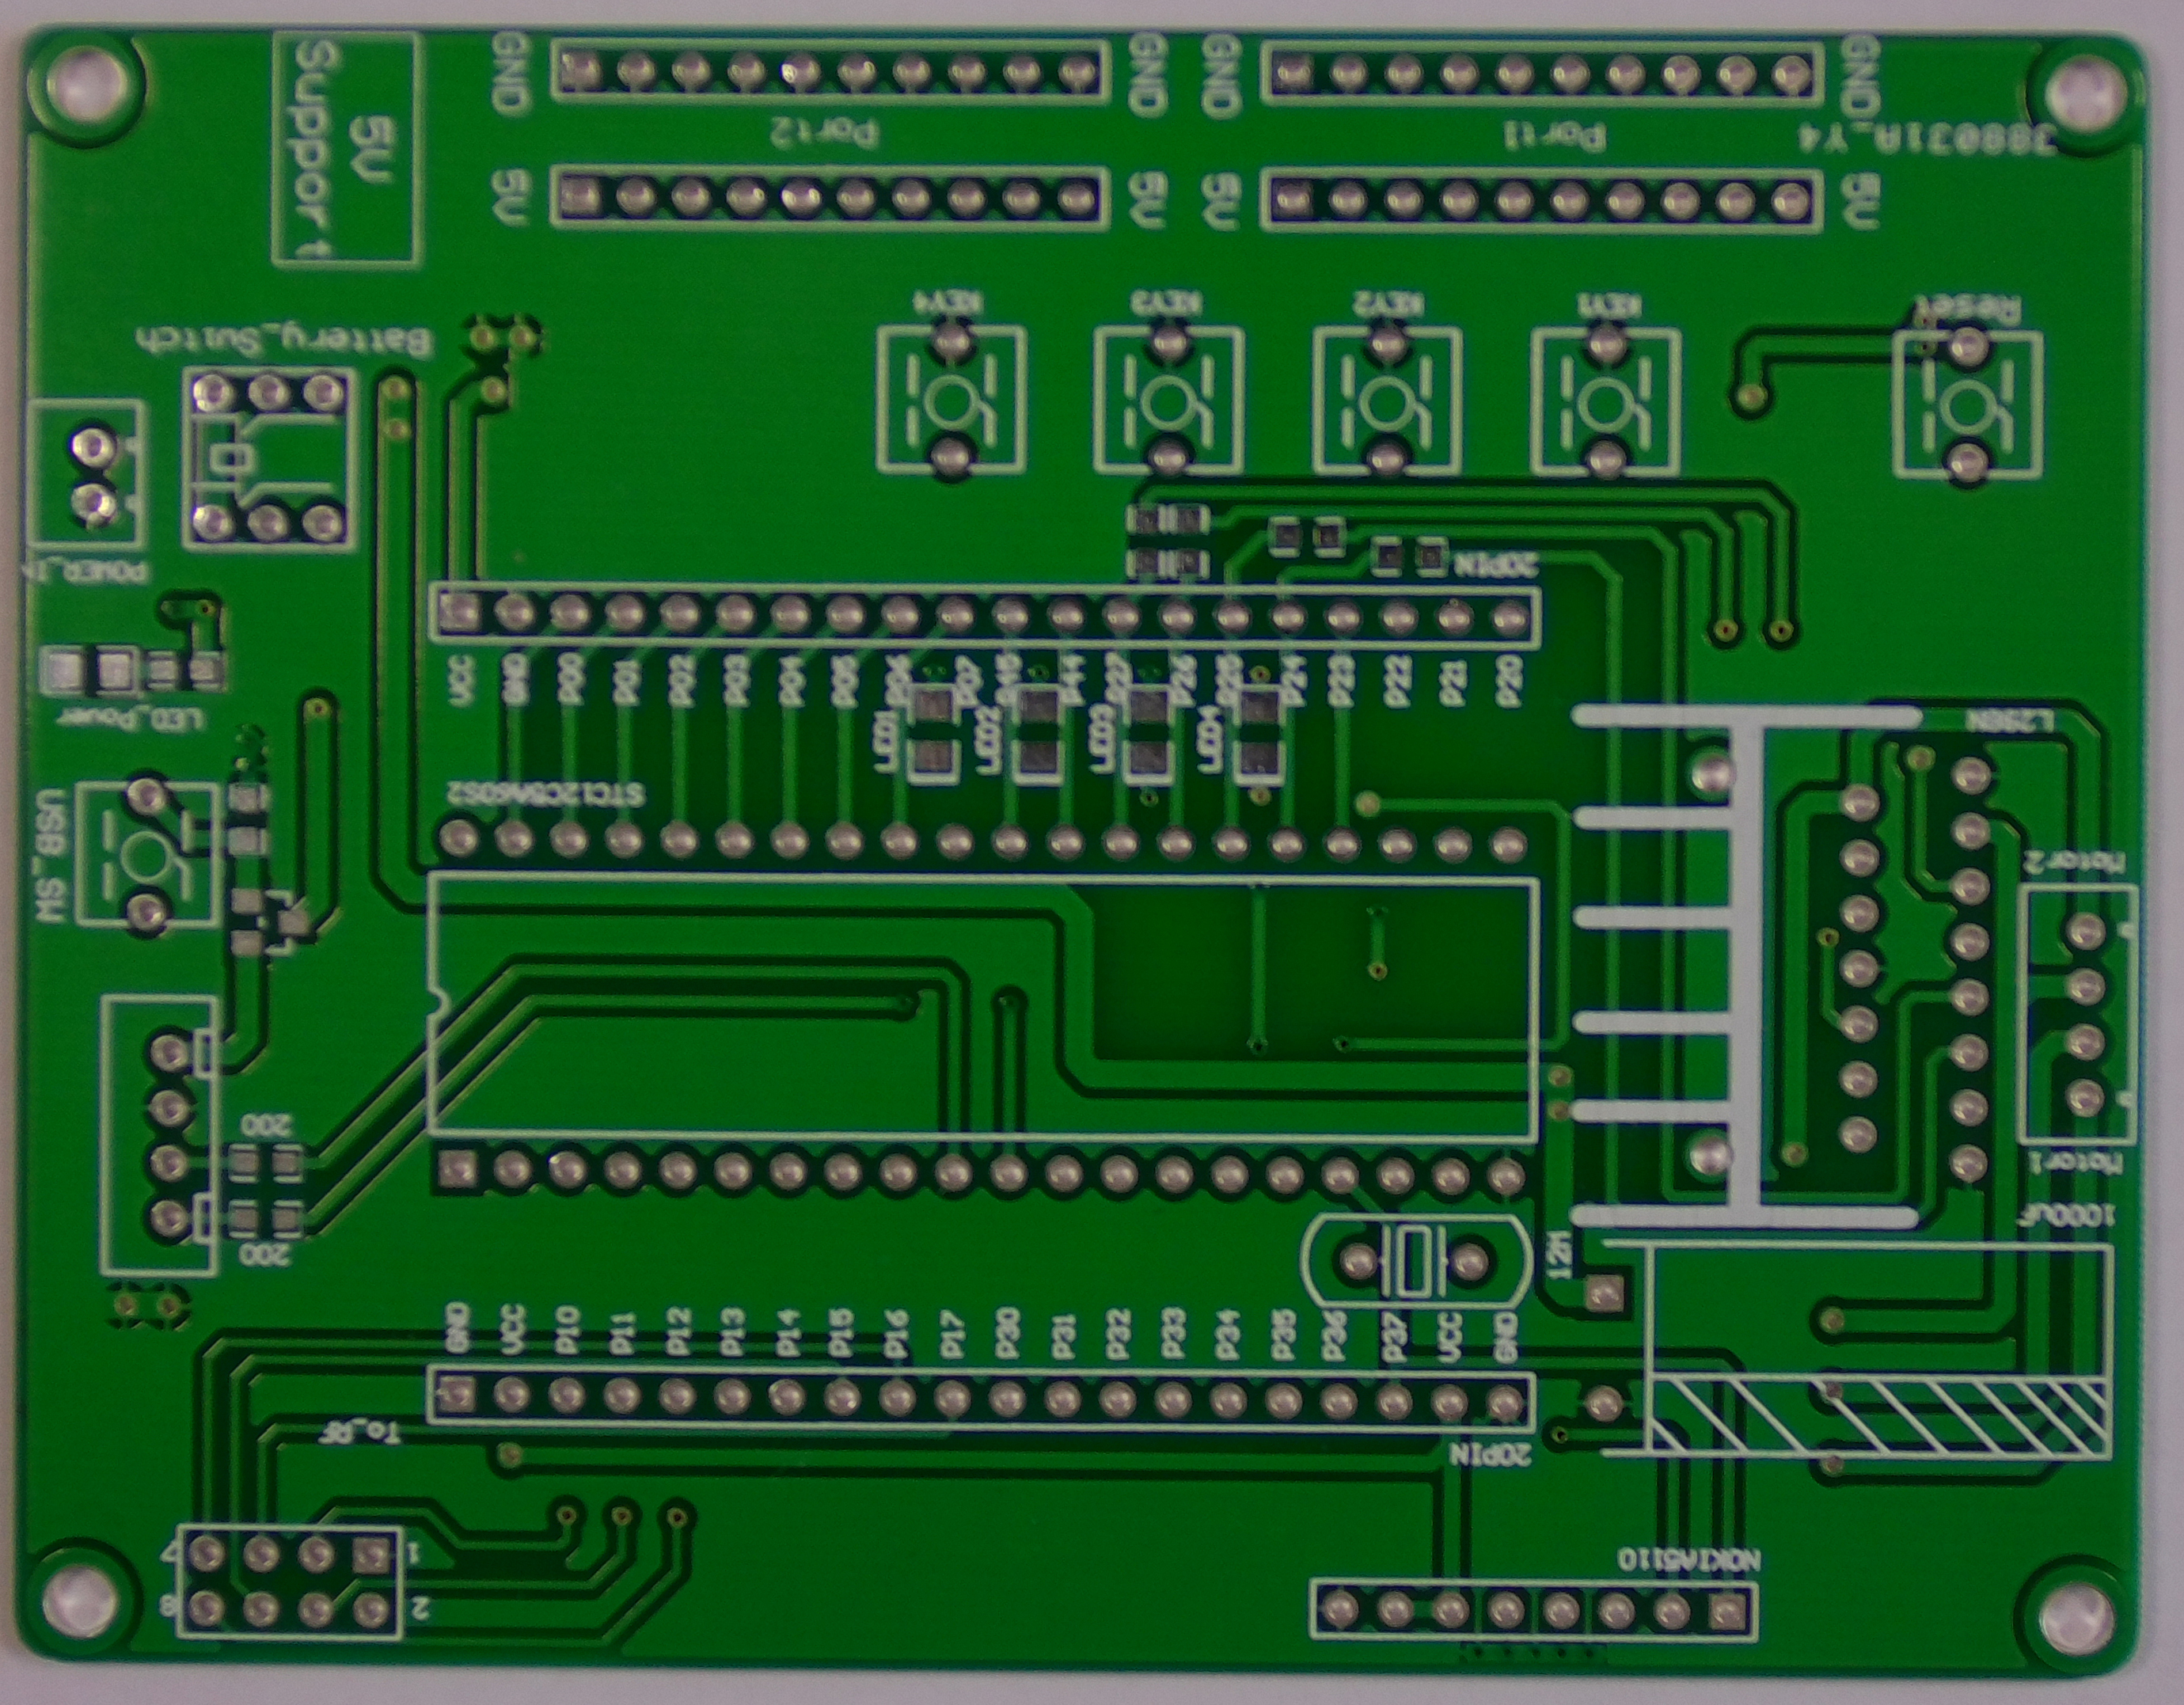
\includegraphics[scale=0.13]{img/pcbs/08.JPG}
  \label{fig:ap-pcbs-8}
  \indentedfont[15.2cm]{\citeonline{ref:Huang-et-al}}
\end{figure}

\begin{figure}[!h] %H
  \centering
  \caption{PCI Número 09 do conjunto de dados HRIPCB.}
  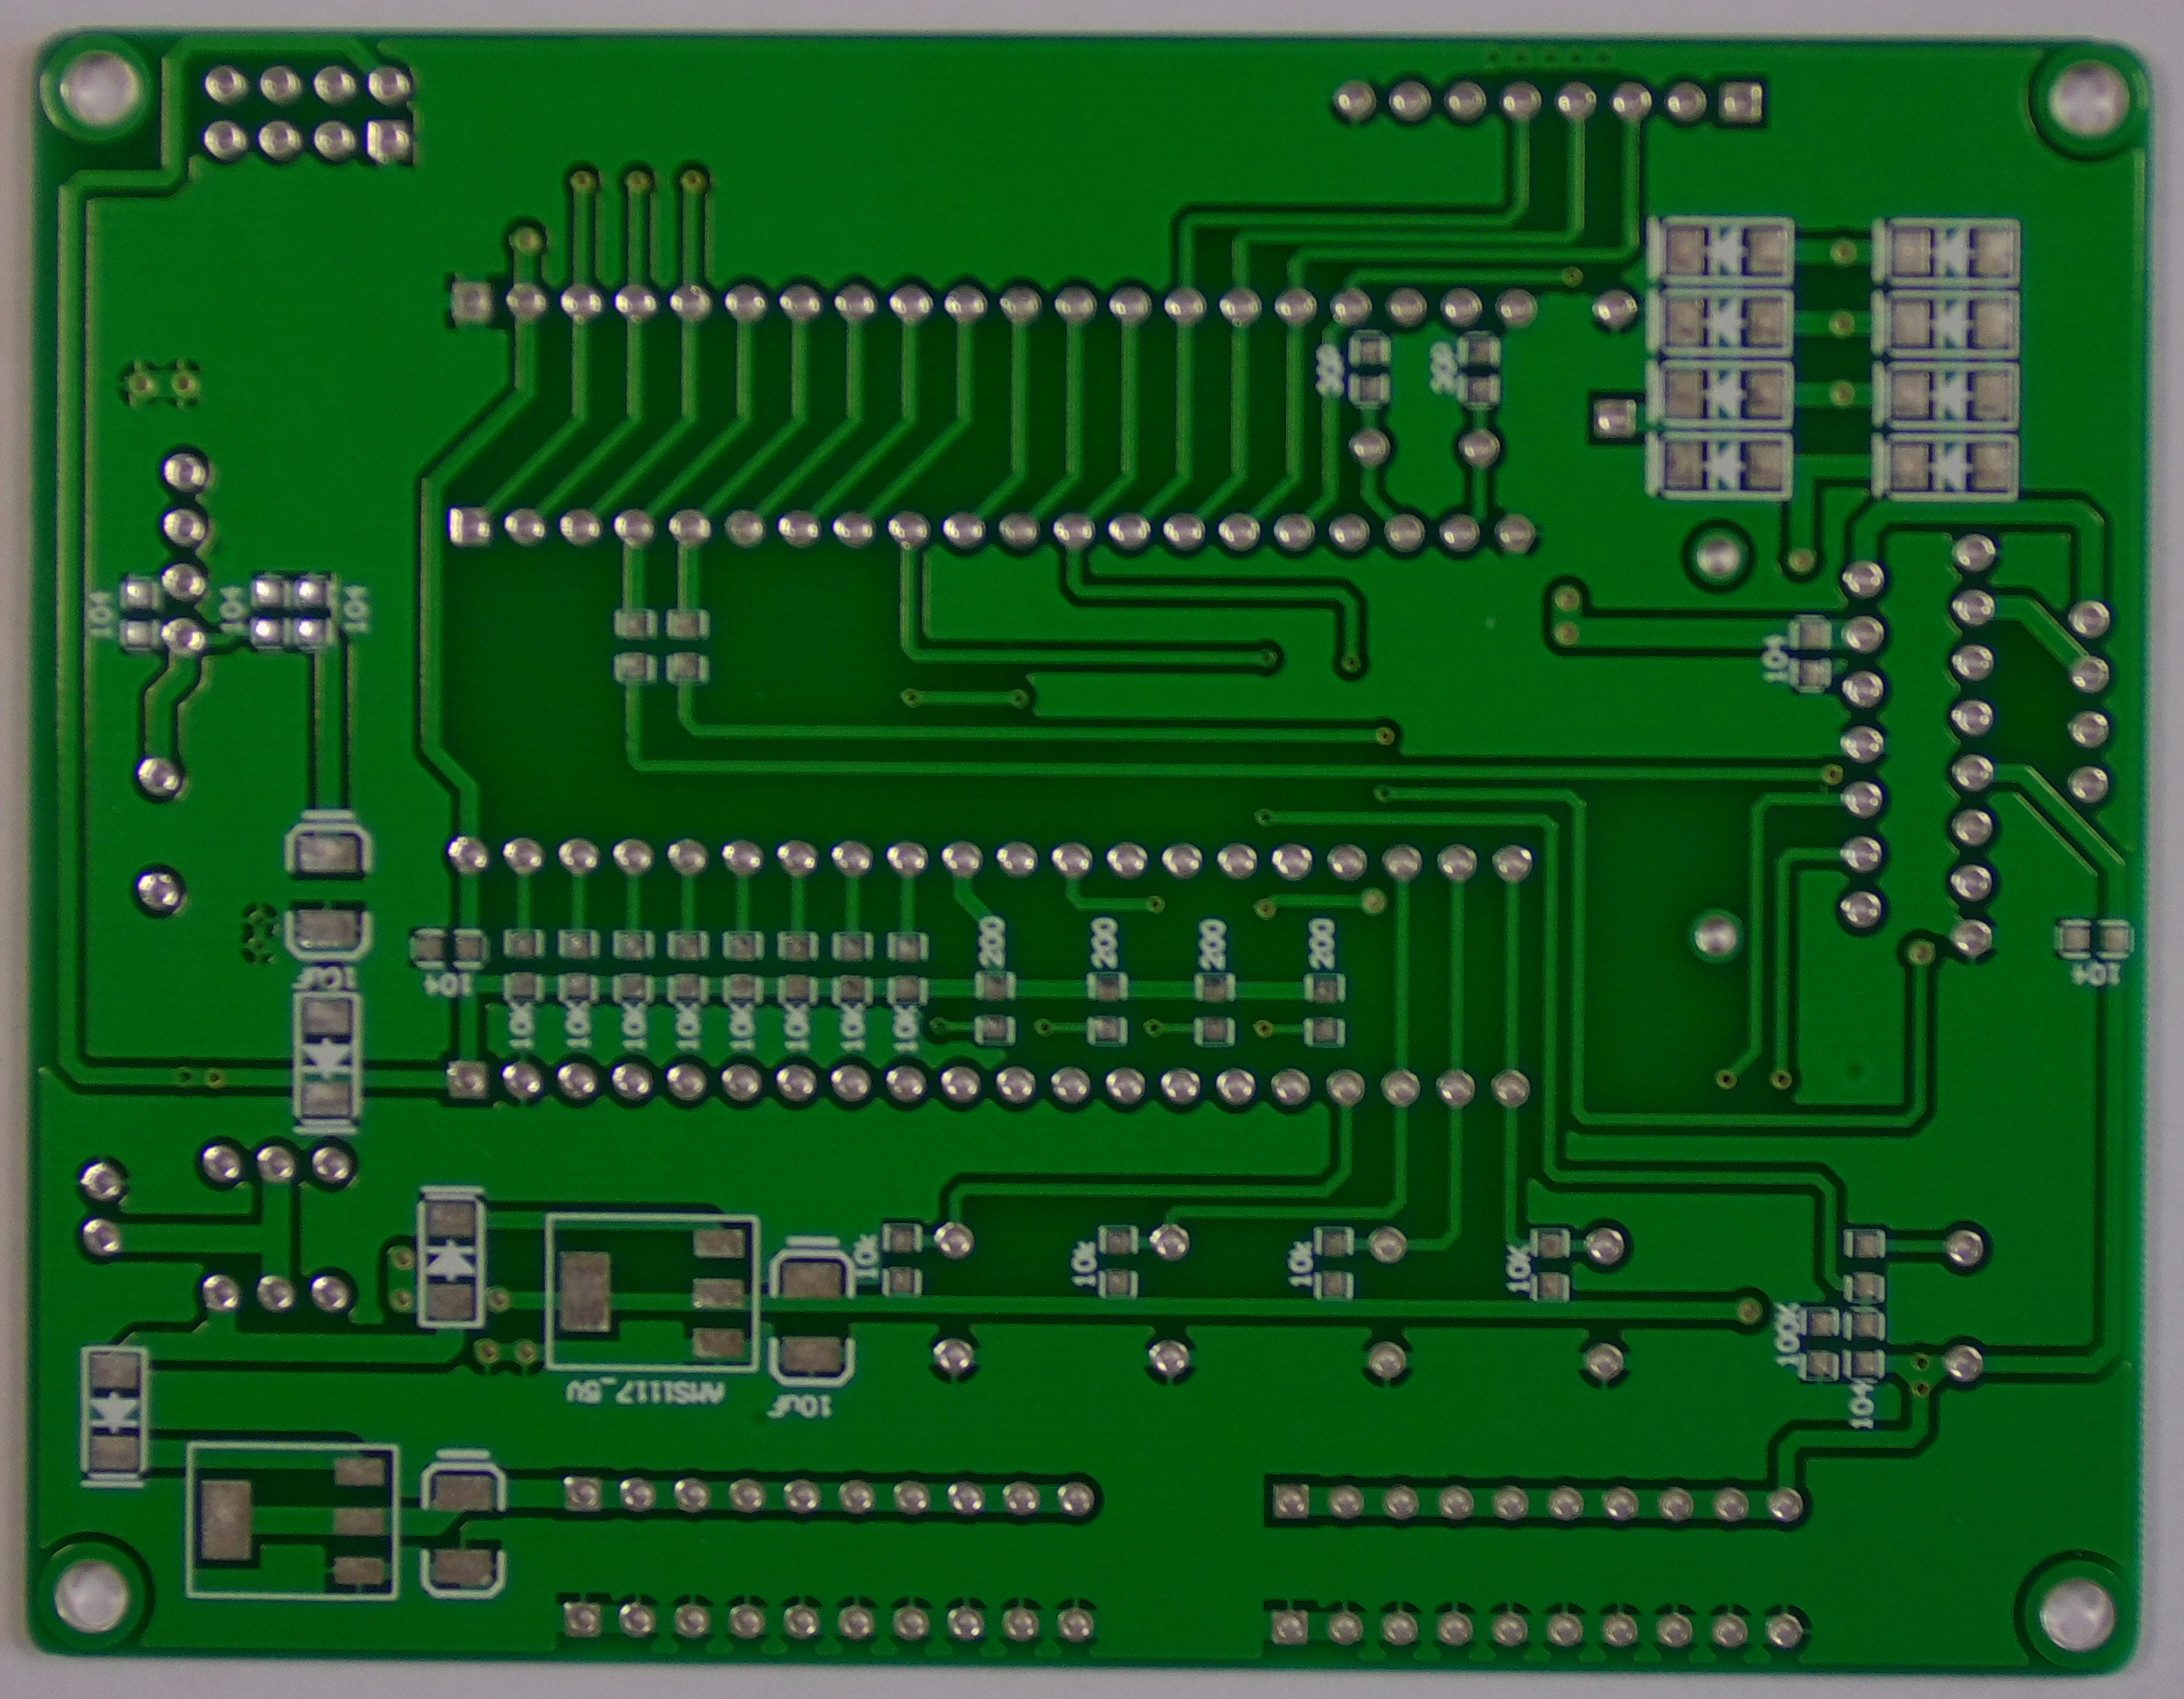
\includegraphics[scale=0.13]{img/pcbs/09.JPG}
  \label{fig:ap-pcbs-9}
  \indentedfont[15.2cm]{\citeonline{ref:Huang-et-al}}
\end{figure}

\begin{figure}[!h] %H
  \centering
  \caption{PCI Número 10 do conjunto de dados HRIPCB.}
  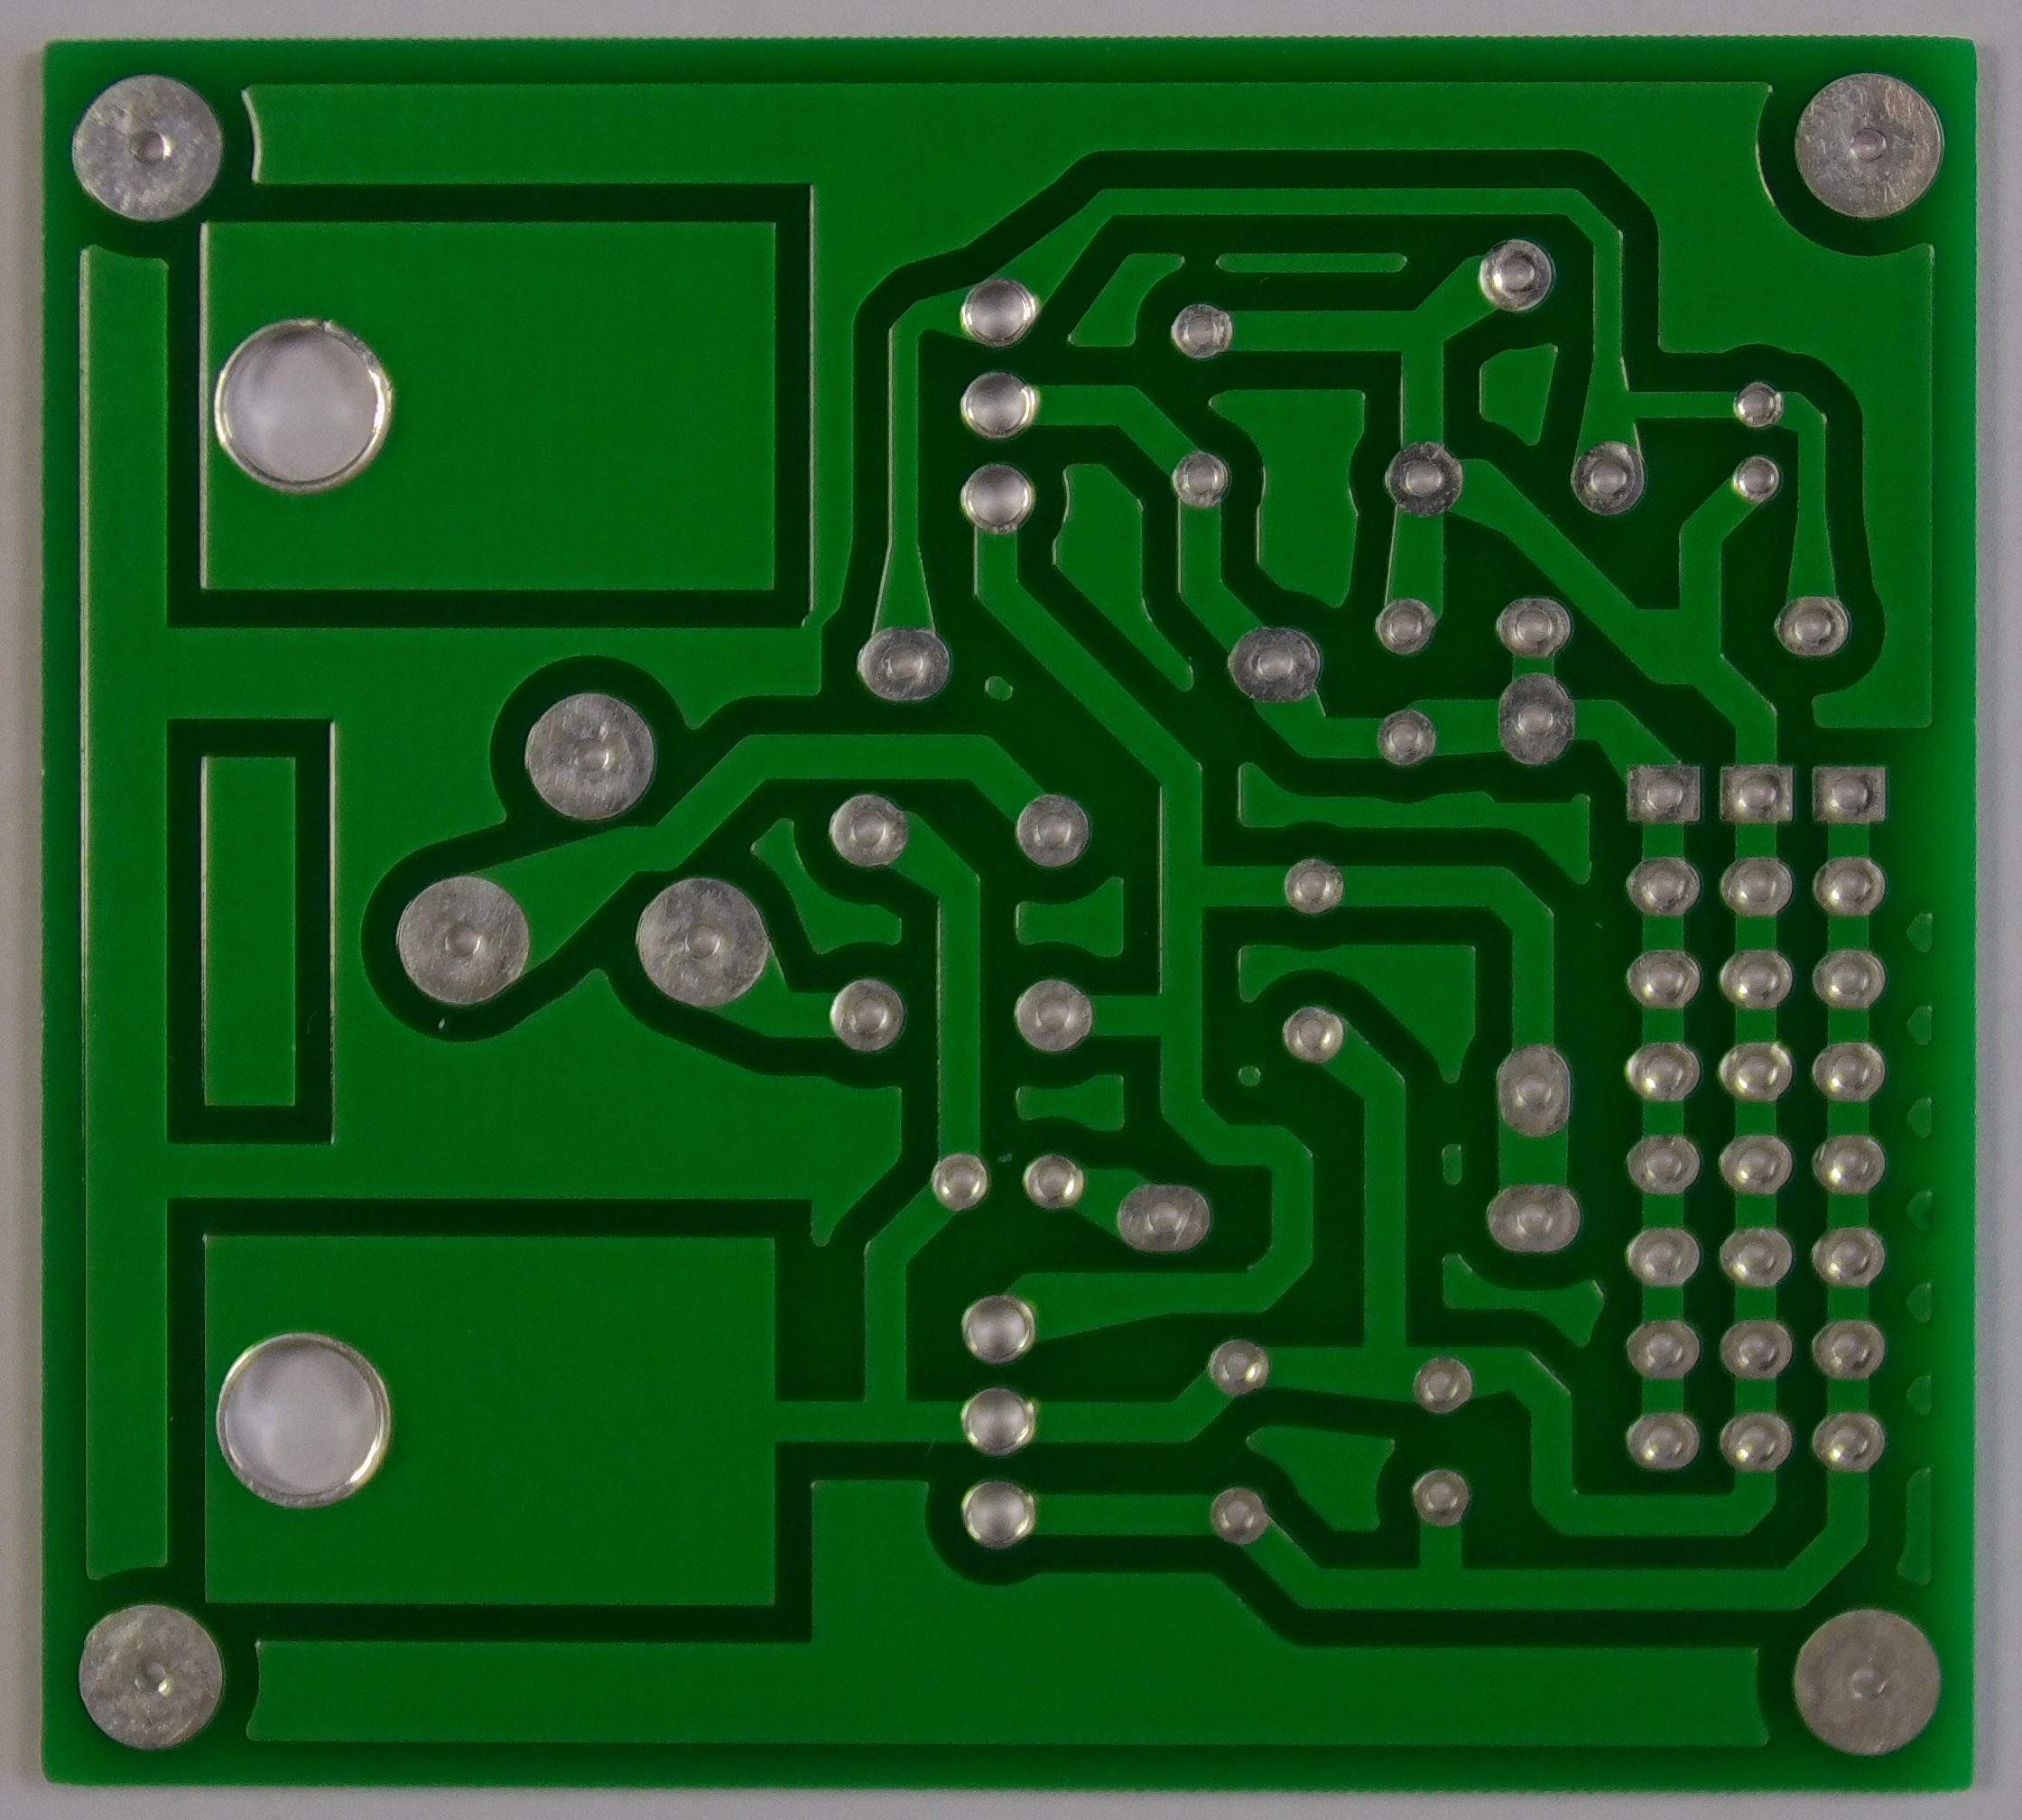
\includegraphics[scale=0.13]{img/pcbs/10.JPG}
  \label{fig:ap-pcbs-10}
  \indentedfont[15.2cm]{\citeonline{ref:Huang-et-al}}
\end{figure}

\begin{figure}[!h] %H
  \centering
  \caption{PCI Número 11 do conjunto de dados HRIPCB.}
  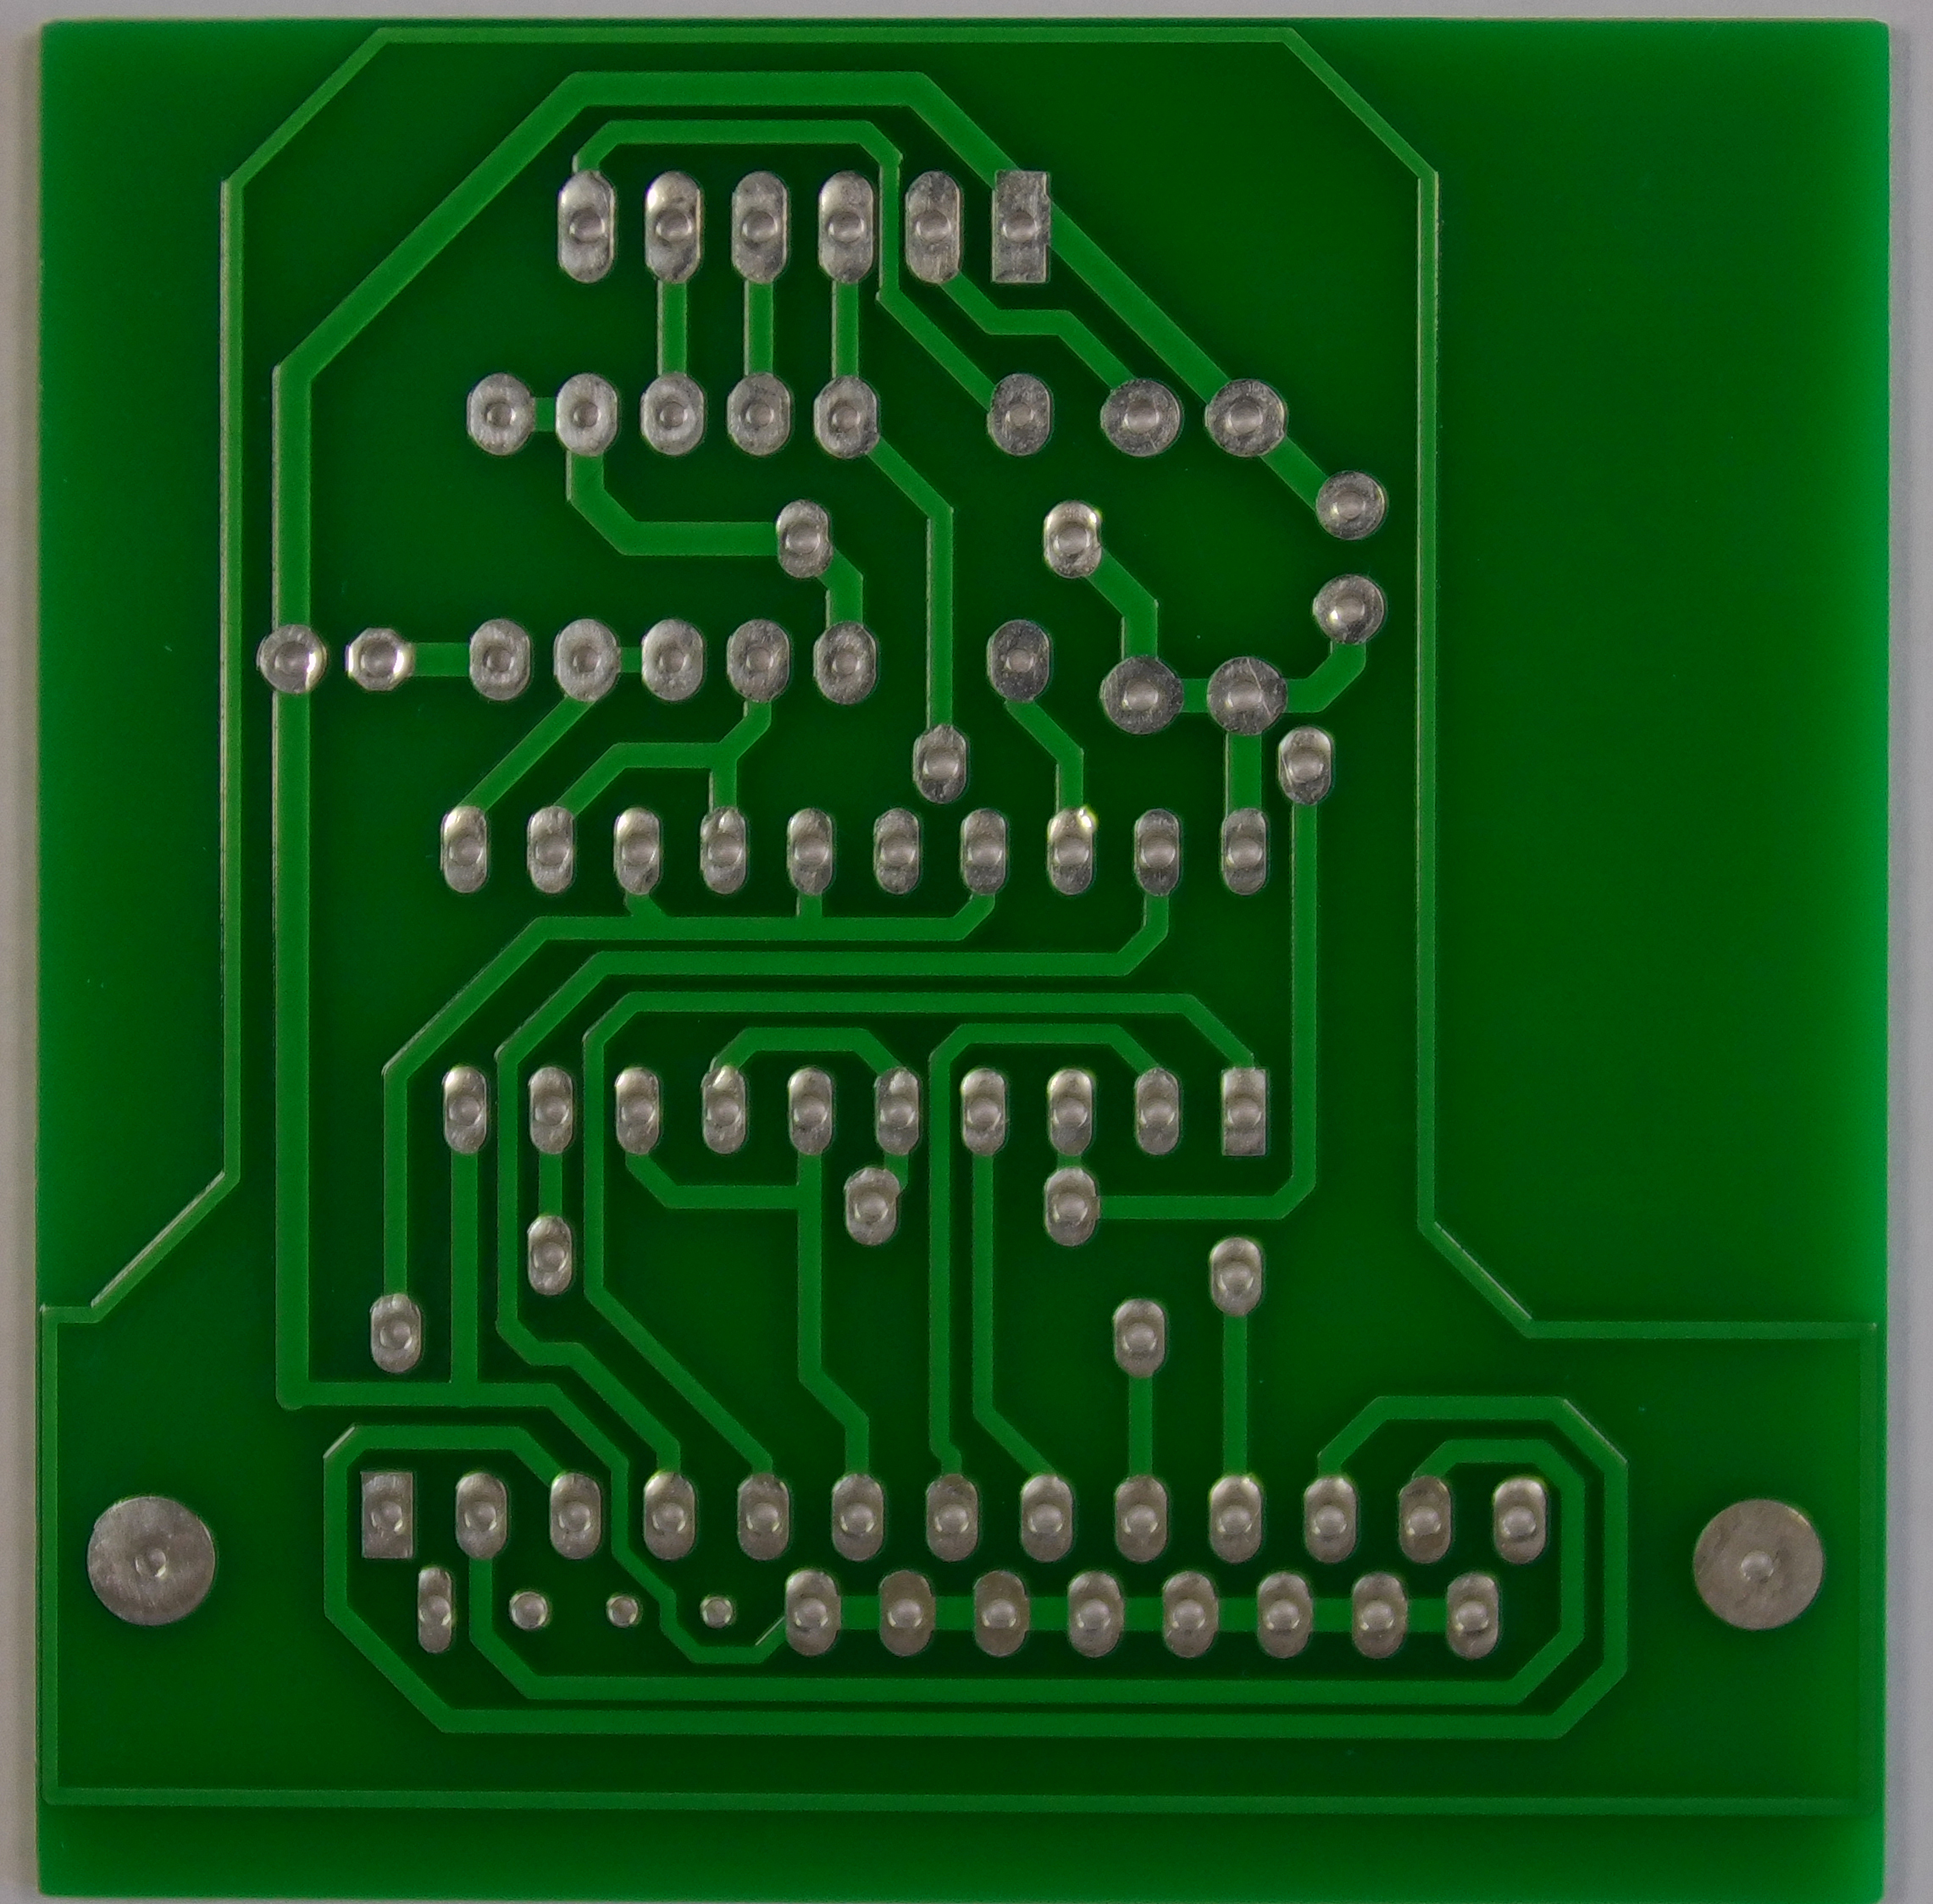
\includegraphics[scale=0.13]{img/pcbs/11.JPG}
  \label{fig:ap-pcbs-11}
  \indentedfont[15.2cm]{\citeonline{ref:Huang-et-al}}
\end{figure}

\begin{figure}[!h] %H
  \centering
  \caption{PCI Número 12 do conjunto de dados HRIPCB.}
  \includegraphics[scale=0.11]{img/pcbs/12.JPG}
  \label{fig:ap-pcbs-12}
  \indentedfont[15.2cm]{\citeonline{ref:Huang-et-al}}
\end{figure}


\chapter{Exemplo de Arquivo de Anotação do Conjunto de Dados HRIPCB em XML} \label{apendice:hripcb-xml}
\lstinputlisting[caption=Arquivo de Anotação do \textit{Dataset} HRIPCB., label=lst:hripcb, firstnumber=1, language=XML]{cod/anotacoes-HRIPCB.xml}

\chapter{\textit{Script} Utilizado na Conversão dos Arquivos de Anotação} \label{apendice:conversao}
\lstinputlisting[caption=\textit{Script} para conversão de arquivos de anotação de xml pata txt., label=lst:conversao, firstnumber=1, language=Python]{cod/HRIPCB_yolo_dataset_config.py}

\chapter{\textit{Script} Utilizado na Divisão do \textit{Dataset} para Treinamento da Rede Neural} \label{apendice:divisao}
\lstinputlisting[caption=\textit{Script} para divisão do \textit{dataset}., label=lst:conversao, firstnumber=1, language=Python]{cod/dataset_split.py}

\chapter{Código Utilizado para o Treinamento da Rede Neural no Ambiente Google Colab} \label{apendice:treinamento}
\lstinputlisting[caption=Comandos executados no ambiente Google Colab para o treinamento da Rede Neural., label=lst:treinamento, firstnumber=1, language=Python]{cod/treinamento.py}

\chapter{Configurações Para a Execução da Interface de Aplicação De Detecção de Defeitos em Placas de Circuito Impresso} \label{apendice:conf-api}

\lstinputlisting[caption=Compilando o Darknet, label=lst:conf-api, firstnumber=1]{cod/api-config.md}

\lstinputlisting[caption=Executando a Interface de Aplicação, label=lst:conf-api, firstnumber=1]{cod/api-config-2.md}
%\markdownInput{cod/README.md}



%\chapter{Arquivos de Configuração para o Treinamento com YOLOv4 utilizando Darknet} \label{apendice:treinamento-cfg}
%\lstinputlisting[label=lst:treinamento, firstnumber=1]{cod/yolov4_custom.cfg}
